\begin{titlepage}

\chapter{Fundamentación teórica}
\section{Consumo energético}
\subsection{Consumo energético en el hogar}
\subsubsection{Contadores inteligentes}
A día de hoy la mayoría de las compañías eléctricas están sustituyendo los contadores en todas las viviendas por nuevos contadores inteligentes que te muestran el consumo eléctrico de toda la vivienda en tiempo real.\\

Ventajas:
\begin{itemize}
	\item En teoría, la renovación de los contadores corre a cargo de las compañías eléctricas, por lo que esta opción no tiene ningún coste extra.
\end{itemize}
Inconvenientes:
\begin{itemize}
	\item La medida que nos da es genérica y no podemos saber cual es el consumo individual de ciertos dispositivos en nuestra red.
	\item En algunos bloques de viviendas, los contadores no se encuentran dentro de las viviendas si no en zonas comunes, por lo que no es tan fácil consultar los datos.
\end{itemize}
\begin{figure}[h!]
	\centering
	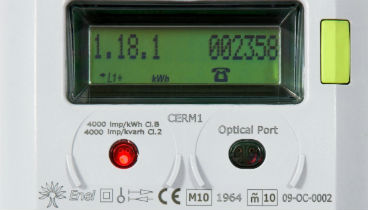
\includegraphics[width=0.75\textwidth]{imagenes/contador.jpg}
	\caption{Contador de luz\cite{contador_img}}
\end{figure}
\subsubsection{Factura de la luz}
En la factura eléctrica podemos consultar el desglose del consumo general por tramos.\\

Ventajas:
\begin{itemize}
	\item Desglose por tarifas del consumo.
\end{itemize}
Inconvenientes:
\begin{itemize}
	\item No podemos conocer en tiempo real el consumo eléctrico de la vivienda.
	\item No podemos saber cuál es el consumo individual de dispositivos en nuestra red.
\end{itemize}
%\begin{figure}[h!]
%	\centering
%	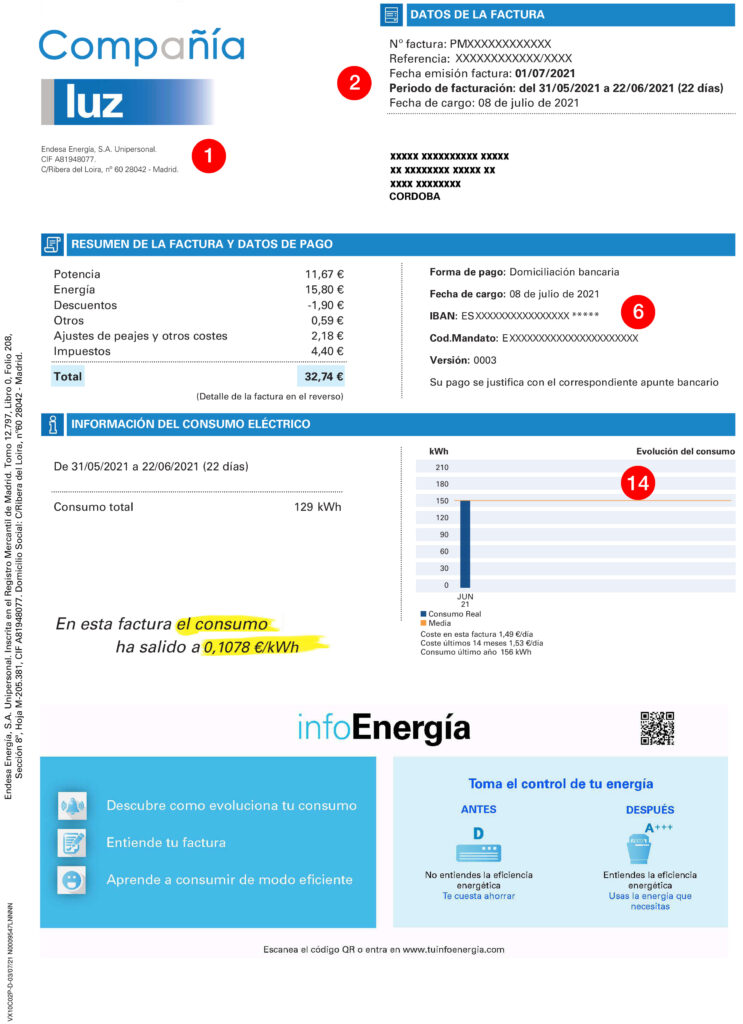
\includegraphics[width=1\textwidth]{imagenes/factura_luz.jpg}
%	\caption{Ejemplo factura de la luz\cite{factura_img}}
%\end{figure}

\subsubsection{Calculo manual del consumo}
Podemos calcular cuánto gasta un dispositivo de manera fácil conociendo su potencia y el tiempo que está encendido. Mas adelante veremos mas en profundidad como hacerlo de diferentes formas.\\

Inconvenientes:\\
\begin{itemize}
	\item Solo es posible saber el consumo teórico.
\end{itemize}

\subsubsection{Medidor de consumo electrico individual}
Medidor de consumo para monitorizar la energía de un dispositivo conectado a la red eléctrica.\\

Ventajas:
\begin{itemize}
	\item Protección por sobrecarga eléctrica incorporado.
	\item Pantalla incorporada para mostrar la lectura.
\end{itemize}

Inconvenientes:
\begin{itemize}
	\item No es posible utilizar los datos de consumo fuera de la pantalla incorporada.
	\item No es posible consultar un historico de consumo.
\end{itemize}
\begin{figure}[h!]
	\centering
	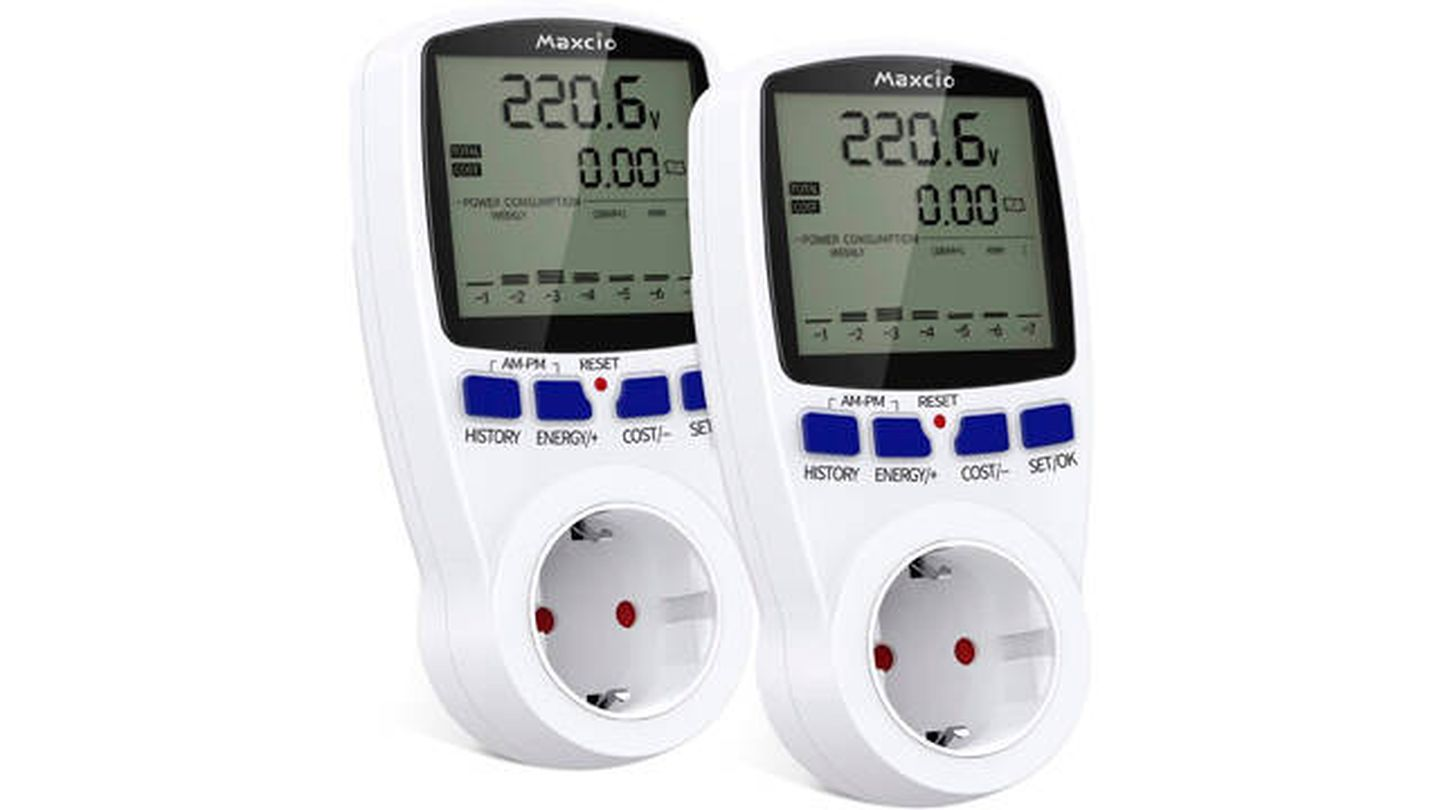
\includegraphics[width=0.5\textwidth]{imagenes/medidor_consumo.jpg}
	\caption{Medidor de consumo de energía\cite{medidor_img}}
\end{figure}

\subsubsection{Medidor cuadro electrico}
Permite medir la energía eléctrica de manera precisa y fiable.\\

Ventajas:
\begin{itemize}
	\item Está pensado para instalarse directamente en el cuadro eléctrico.
	\item Permite medir amperajes muy altos.
\end{itemize}

Inconvenientes:
\begin{itemize}
	\item Al instalarse en el cuadro eléctrico, la medida que nos da es genérica y no podemos saber cual es el consumo individual de ciertos dispositivos en nuestra red electrica. 
\end{itemize}
\begin{figure}[h!]
	\centering
	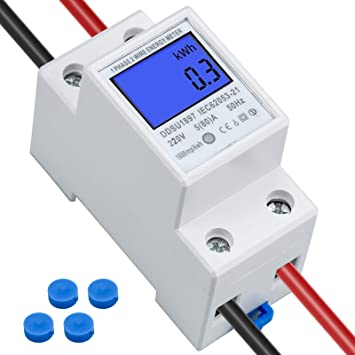
\includegraphics[width=0.25\textwidth]{imagenes/medidor_cuadro.jpg}
	\caption{Medidor de consumo en cuadro electrico\cite{medidor_cuadro_img}}
\end{figure}

\subsubsection{Monitor inteligente de energia}
Sistema que agrega sensores individuales para monitorizar de forma precisa electrodomésticos y otros tipos de dispositivos. Integración con una app Android para consultar los datos. Esta opción sería lo más parecido al sistema que este proyecto plantea.\\

Ventajas:
\begin{itemize}
	\item Sensores de hasta 50A.
	\item Cuenta con una aplicación para consultar los datos de cada sensor.
\end{itemize}

Inconvenientes:
\begin{itemize}
	\item Los sensores se comunican con el panel principal por cable.
	\item Coste elevado.
\end{itemize}
\begin{figure}[h!]
	\centering
	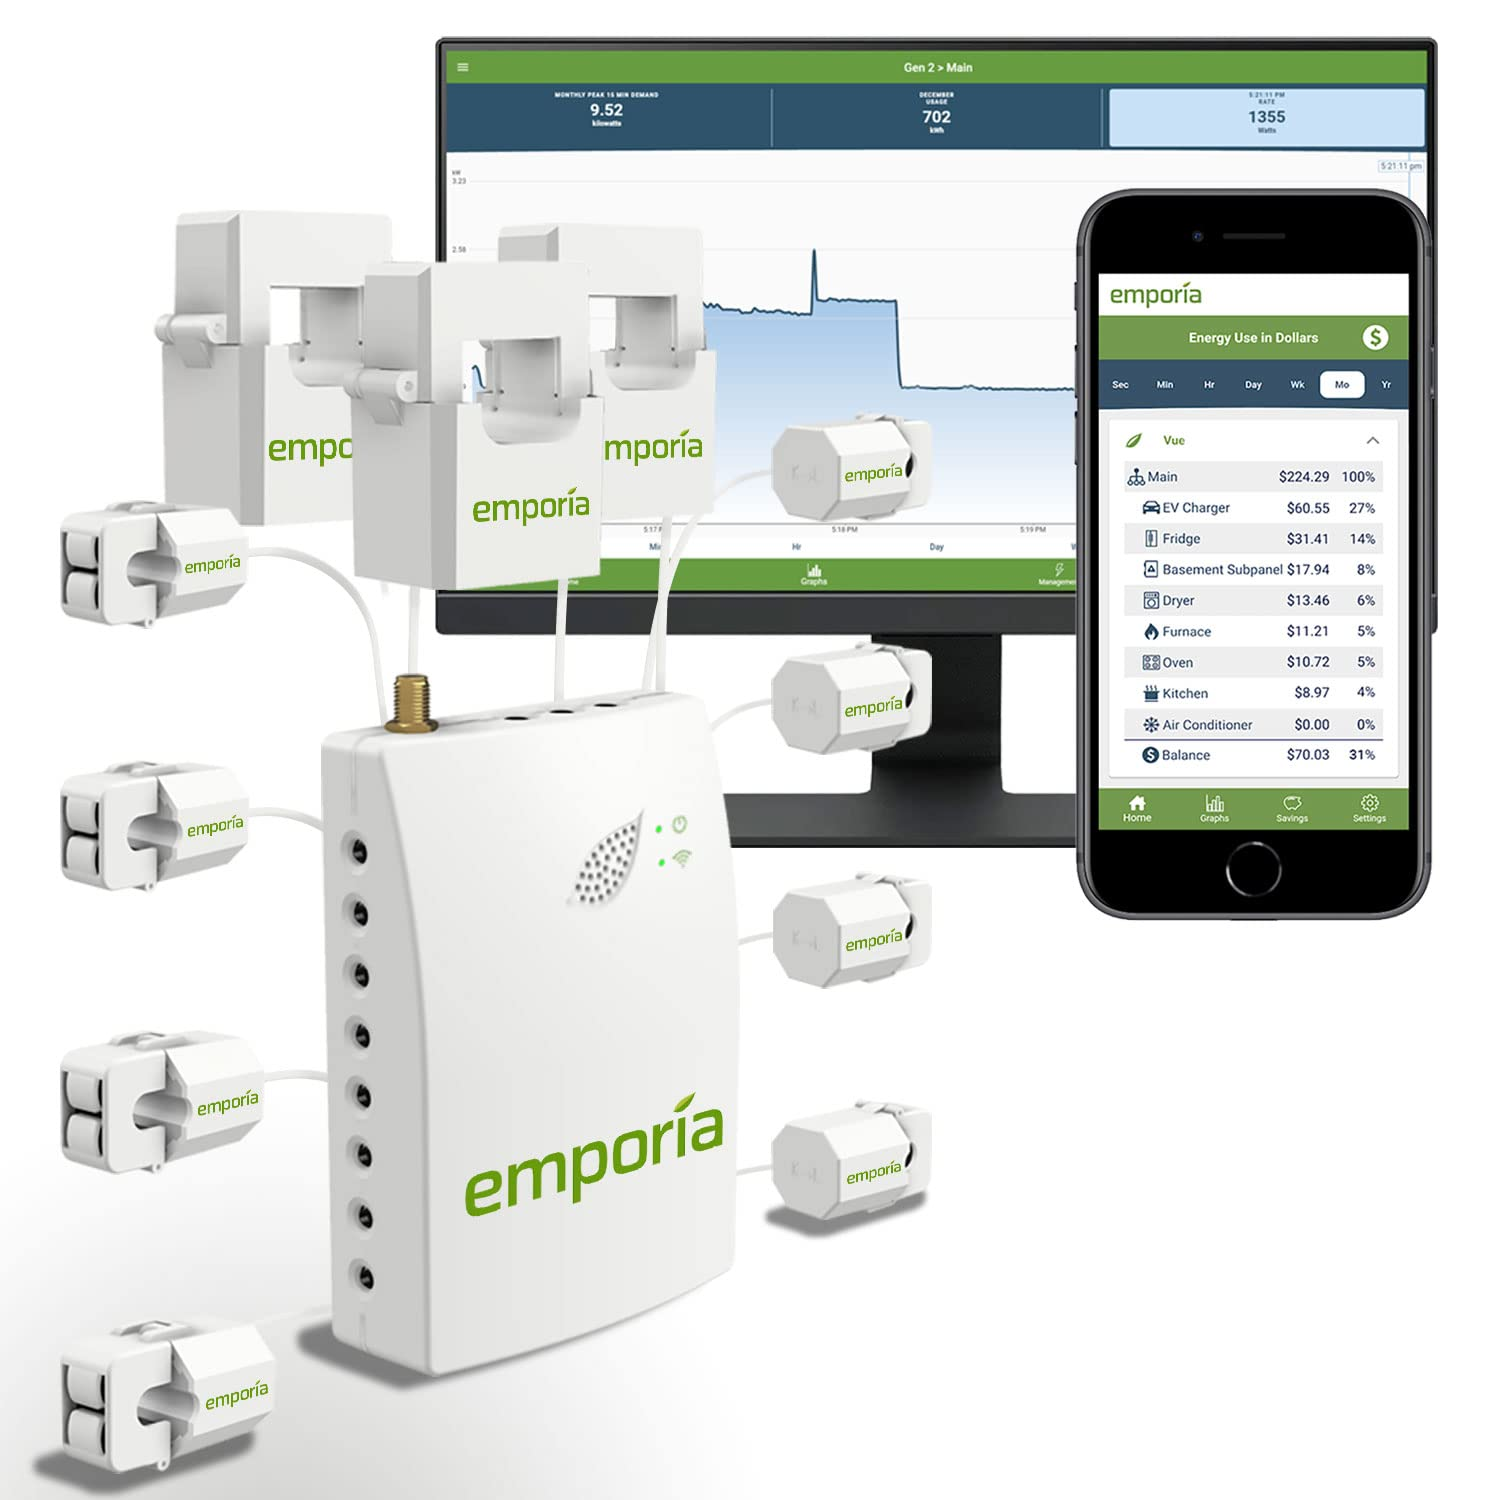
\includegraphics[width=0.25\textwidth]{imagenes/monitor_consumo.jpg}
	\caption{Monitor de energia inteligente\cite{monitor_inteligente_img}}
\end{figure}

\newpage

\subsection{Calculo del consumo energético}
Lo primero que necesitamos entender es como podemos calcular el consumo electrico de cualquier dispositvo. Sabiendo los datos teoricos, es algo bastante simple, tan solo necesitamos aplicar la siguiente formula: \\
\begin{equation}
\label{eq:consumo}
P = I \cdot V
\end{equation}

Donde P es el consumo en vatios, I es la intensidad en amperios y V es la tensión en voltios. La tensión es facil saberla. En España y en la mayoria de paises europeos, la tensión es de 230V. Pero la intensidad es algo mas complicado. Para saber la intensidad necesitamos saber la potencia del dispositivo. Para ello, podemos consultar la etiqueta de consumo de cada dispositivo. En la etiqueta de consumo, podemos ver la potencia en vatios, la intensidad en amperios y la tensión en voltios. Pero esta potencia que nos indica el dispositivo no es la real. Normalmente es la potencia maxima que puede llegar a consumir el dispositivo, pero no la que realmente consume. Para calcular la potencia real, podemos hacer uso de un multimetro y asi obtener la intensidad real, y con esto calcular la potencia que consume. En nuestra solución no podremos hacer uso de un multimetro, asi que necesitamos entender como hace el multimetro para calcular la intensidad. \\

\subsubsection{Onda sinusoidal}
La corriente alterna viaja por el cableado en formas de ondas Sinusoidales. La forma de onda de la corriente alterna es la siguiente: \\ 

\begin{figure}[h!]
	\centering
	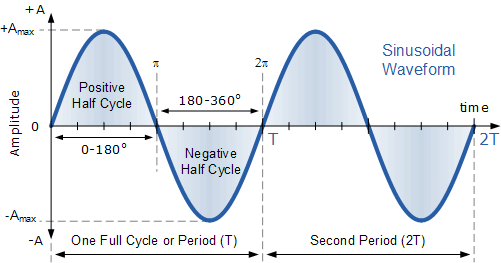
\includegraphics[width=0.75\textwidth]{imagenes/sine_wave.png}
	\caption{Forma de una onda Sinusoidal\cite{sine_wave_img}}
\end{figure}
\newpage
Aquí podemos diferenciar tres caracteristicas de la onda sinusoidal\cite{ref2}: \\
\begin{itemize}
	\item Amplitud: Es la distancia entre el punto mas alto y el mas bajo de la onda. Esta es la intensidad de la señal de corriente.
	\item Frecuencia: Es el numero de veces que la onda se repite en un segundo. En España, la frecuencia es de 50Hz.
	\item Periodo: Es el tiempo que tarda en completarse una onda.
\end{itemize}
Para poder calcular correctamente el consumo de un dispositivo, tenemos que medir correctamente la amplitud de la onda, es decir, el maximo y minimo de la onda. Asi es como los amperimetros y los multimetros calculan la intensidad. \\
\subsubsection{Factor de potencia}
El factor de potencia\cite{ref3} se utiliza como expresión para indicar la relación entre la potencia activa y la potencia aparente. La potencia aparente es la potencia que se mide en el medidor de la compañia electrica. La potencia activa es la potencia que realmente consume el dispositivo. Si un circuito electrico fuera cien por cien eficiente, la potencia activa y la potencia aparente serian iguales. Pero en la realidad, los circuitos no son cien por cien eficientes, y por tanto, la potencia activa es menor que la potencia aparente. \\
\begin{equation}
\label{eq:factor_potencia}
FP = \frac{P_{activa}}{P_{aparente}}
\end{equation}
El factor de potencia es un valor que oscila entre 0 y 1. Cuanto mas cercano a 1, mas eficiente es el circuito. Cuanto mas cercano a 0, menos eficiente es el circuito. En aparatos electricos resistivos (como por ejemplo un radiador), el factor de potencia es muy cercano a 1 ya que convierten toda la energia electrica que reciben en calor. En aparatos electricos inductivos, como por ejemplo un motor, el factor de potencia es mucho mas bajo ya que no convierten toda la energia electrica que reciben en trabajo.

\subsubsection{Media cuadratica (RMS)}
Para este proyecto, no nos interesa el el peak-to-peak de la onda, sino la media cuadratica\cite{ref4} de la onda para poder saber la intensidad continua que consume el dispositivo. Para calcular la media cuadratica, podemos hacer uso de la siguiente formula: \\
\begin{equation}
\label{eq:peak_to_peak}
	V_{peak\_to\_peak} = V_{max} - V_{min}
\end{equation}
	
\begin{equation}
\label{eq:media_cuadratica}
Voltage RMS = (\frac{V_{peak\_to\_peak}}{2}) \cdot \sqrt{2}
\end{equation}

\subsection{Sensores de consumo energético}
A continuacion vamos a ver los diferentes tipos de sensores que podemos utilizar para medir el consumo de un dispositivo en nuestro proyecto. \\
\subsubsection{INA219}
El sensor INA219\cite{ref5} es un sensor de corriente y voltaje de alta precision. Este sensor es capaz de medir hasta 26V. Este sensor es muy util para medir el consumo de un dispositivo, ya que es capaz de medir tanto la intensidad como la tensión, como por ejemplo para monitorizar la duración de baterias.\\

Caracteristicas:
\begin{itemize}
	\item Mide tensiones entre 0 y 26V.
	\item Interfaz de comunicación I2C.
	\item Alta precisión.
	\item Opciones de calibración para ajustar la sensibilidad.
\end{itemize}
\begin{figure}[h!]
	\centering
	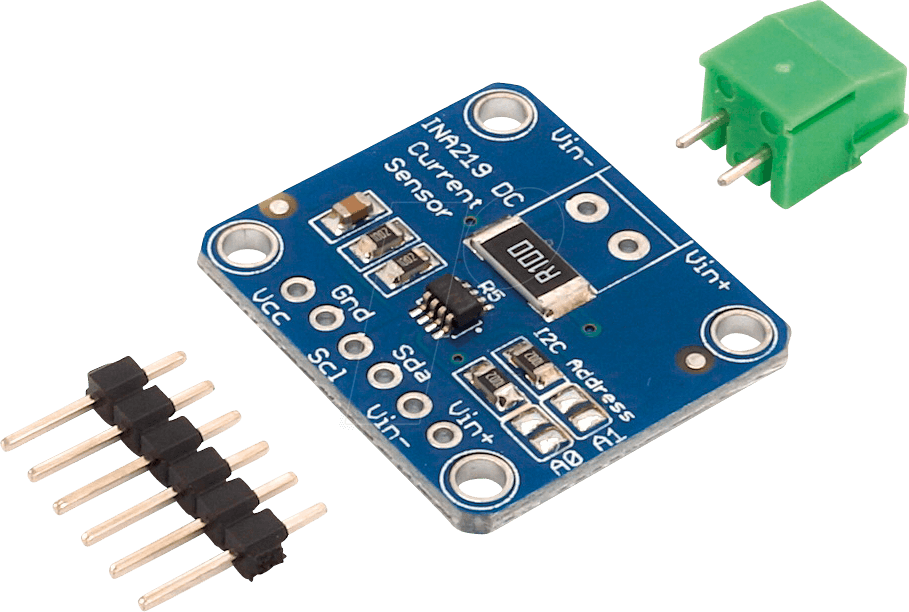
\includegraphics[width=0.25\textwidth]{imagenes/ina219.png}
	\caption{Sensor INA219\cite{ina219_img}}
\end{figure}

\subsubsection{ZMPT101B}
El sensor ZMPT101B\cite{ref6} es capaz de medir hasta 1000V. \\

Caracteristicas:
\begin{itemize}
	\item Alto aislamiento.
	\item Rango amplio
	\item Alta precisión
	\item Resultados estables
\end{itemize}

\begin{figure}[h!]
	\centering
	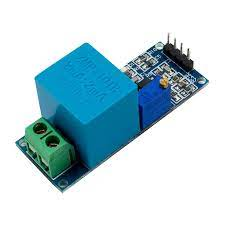
\includegraphics[width=0.25\textwidth]{imagenes/zmpt101b.jpeg}
	\caption{Sensor ZMPT101B\cite{zmpt101b_img}}
\end{figure}


\subsubsection{ACS712}
El sensor ACS712\cite{ref7} es un sensor barato y preciso para medir la corriente tanto continua como alterna. Existen 3 modelos de este sensor, uno para medir corrientes de 5A, otro para medir corrientes de 20A y otro para medir corrientes de 30A. \\

Caracteristicas:
\begin{itemize}
	\item Alta precisión.
	\item Señal de salida con bajo ruido.
\end{itemize}
\begin{figure}[h!]
	\centering
	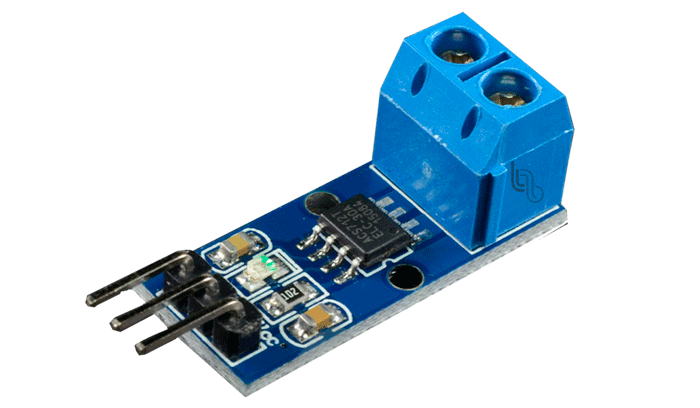
\includegraphics[width=0.25\textwidth]{imagenes/acs712.png}
	\caption{Sensor ACS712\cite{acs712_img}}
\end{figure}

\section{Plataformas de desarrollo}
Para este proyecto, buscamos una plataforma de desarrollo de software embebido que disponga de ADCs y de una interfaz de comunicación inalámbrica para poder enviar los datos a un servidor. A continuación vamos a ver las diferentes opciones que tenemos. \\
\subsection{Arduino}
Arduino\cite{ref8} es una plataforma de desarrollo de software embebido basada en microcontroladores. Arduino es una plataforma muy popular y tiene una gran comunidad de usuarios. Arduino tiene una gran cantidad de shields, que son placas de expansion que se pueden conectar a la placa base de Arduino. No dispone de WiFi integrado, pero podriamos conectarle un modulo WiFi. El Arduino UNO dispone de 6 entradas analogicas. \\
\begin{figure}[h!]
	\centering
	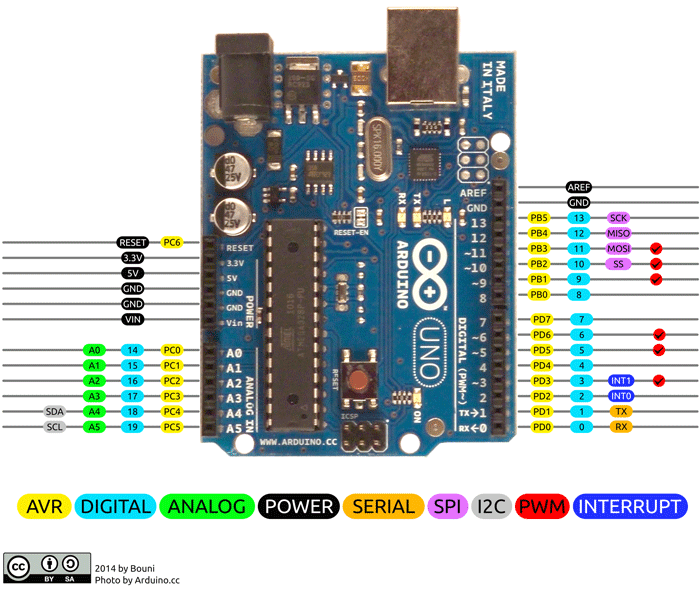
\includegraphics[width=0.5\textwidth]{imagenes/arduino.png}
	\caption{Arduino pin layout\cite{arduino_img}}
\end{figure}
\subsection{Raspberry Pi}
La Raspberry Pi\cite{ref9} es un mini ordenador de bajo coste (aunque mas caro que el resto de plataformas que vamos a ver). No inclute ningun convertidor analogico digital, por lo que tendriamos que usar un modulo externo. Si dispone de WiFi.
\begin{figure}[h!]
	\centering
	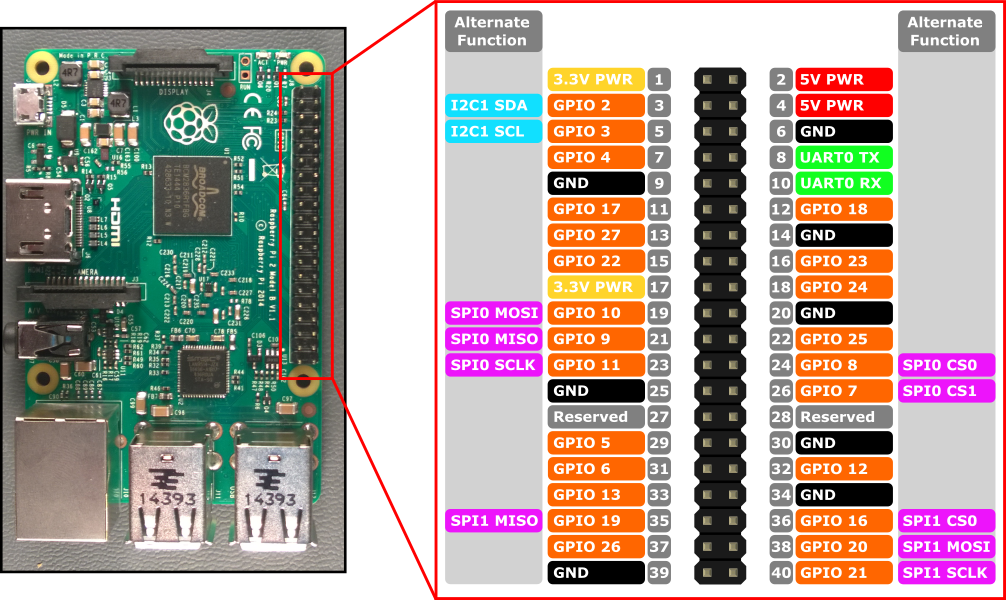
\includegraphics[width=0.5\textwidth]{imagenes/rpi.png}
	\caption{Raspberry Pi pin layout\cite{rpi_img}}
\end{figure}
\subsection{ NodeMCU ESP8266}
El NodeMCU ESP8266\cite{ref10} es una plataforma de codigo abierto que como su propio nombre indica, incluye un modulo WiFi ESP8266. Es un proyecto ya abandonado pero que tiene una gran comunidad de usuarios que lo siguen manteniendo. Esta plataforma tan solo dispone de un ADC, pero de resolución de 10 bits. \\
\begin{figure}[h!]
	\centering
	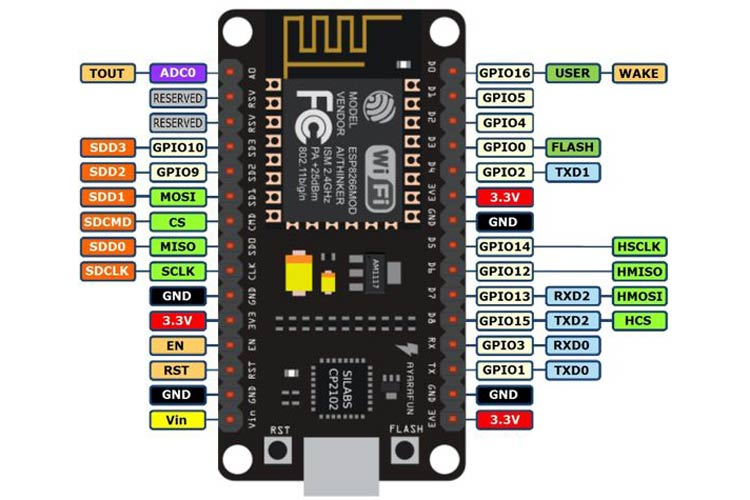
\includegraphics[width=0.5\textwidth]{imagenes/esp8266.jpg}
	\caption{Node MCU ESP8266 pin layout\cite{esp8266_img}}
\end{figure}
\subsection{ESP32}
El ESP32\cite{ref11} es un microcontrolador con WiFi integrado. Dispone de hasta 18 entradas analogicas. Es el sucesor del ESP8266, por lo que es una plataforma mas moderna. \\
\begin{figure}[h!]
	\centering
	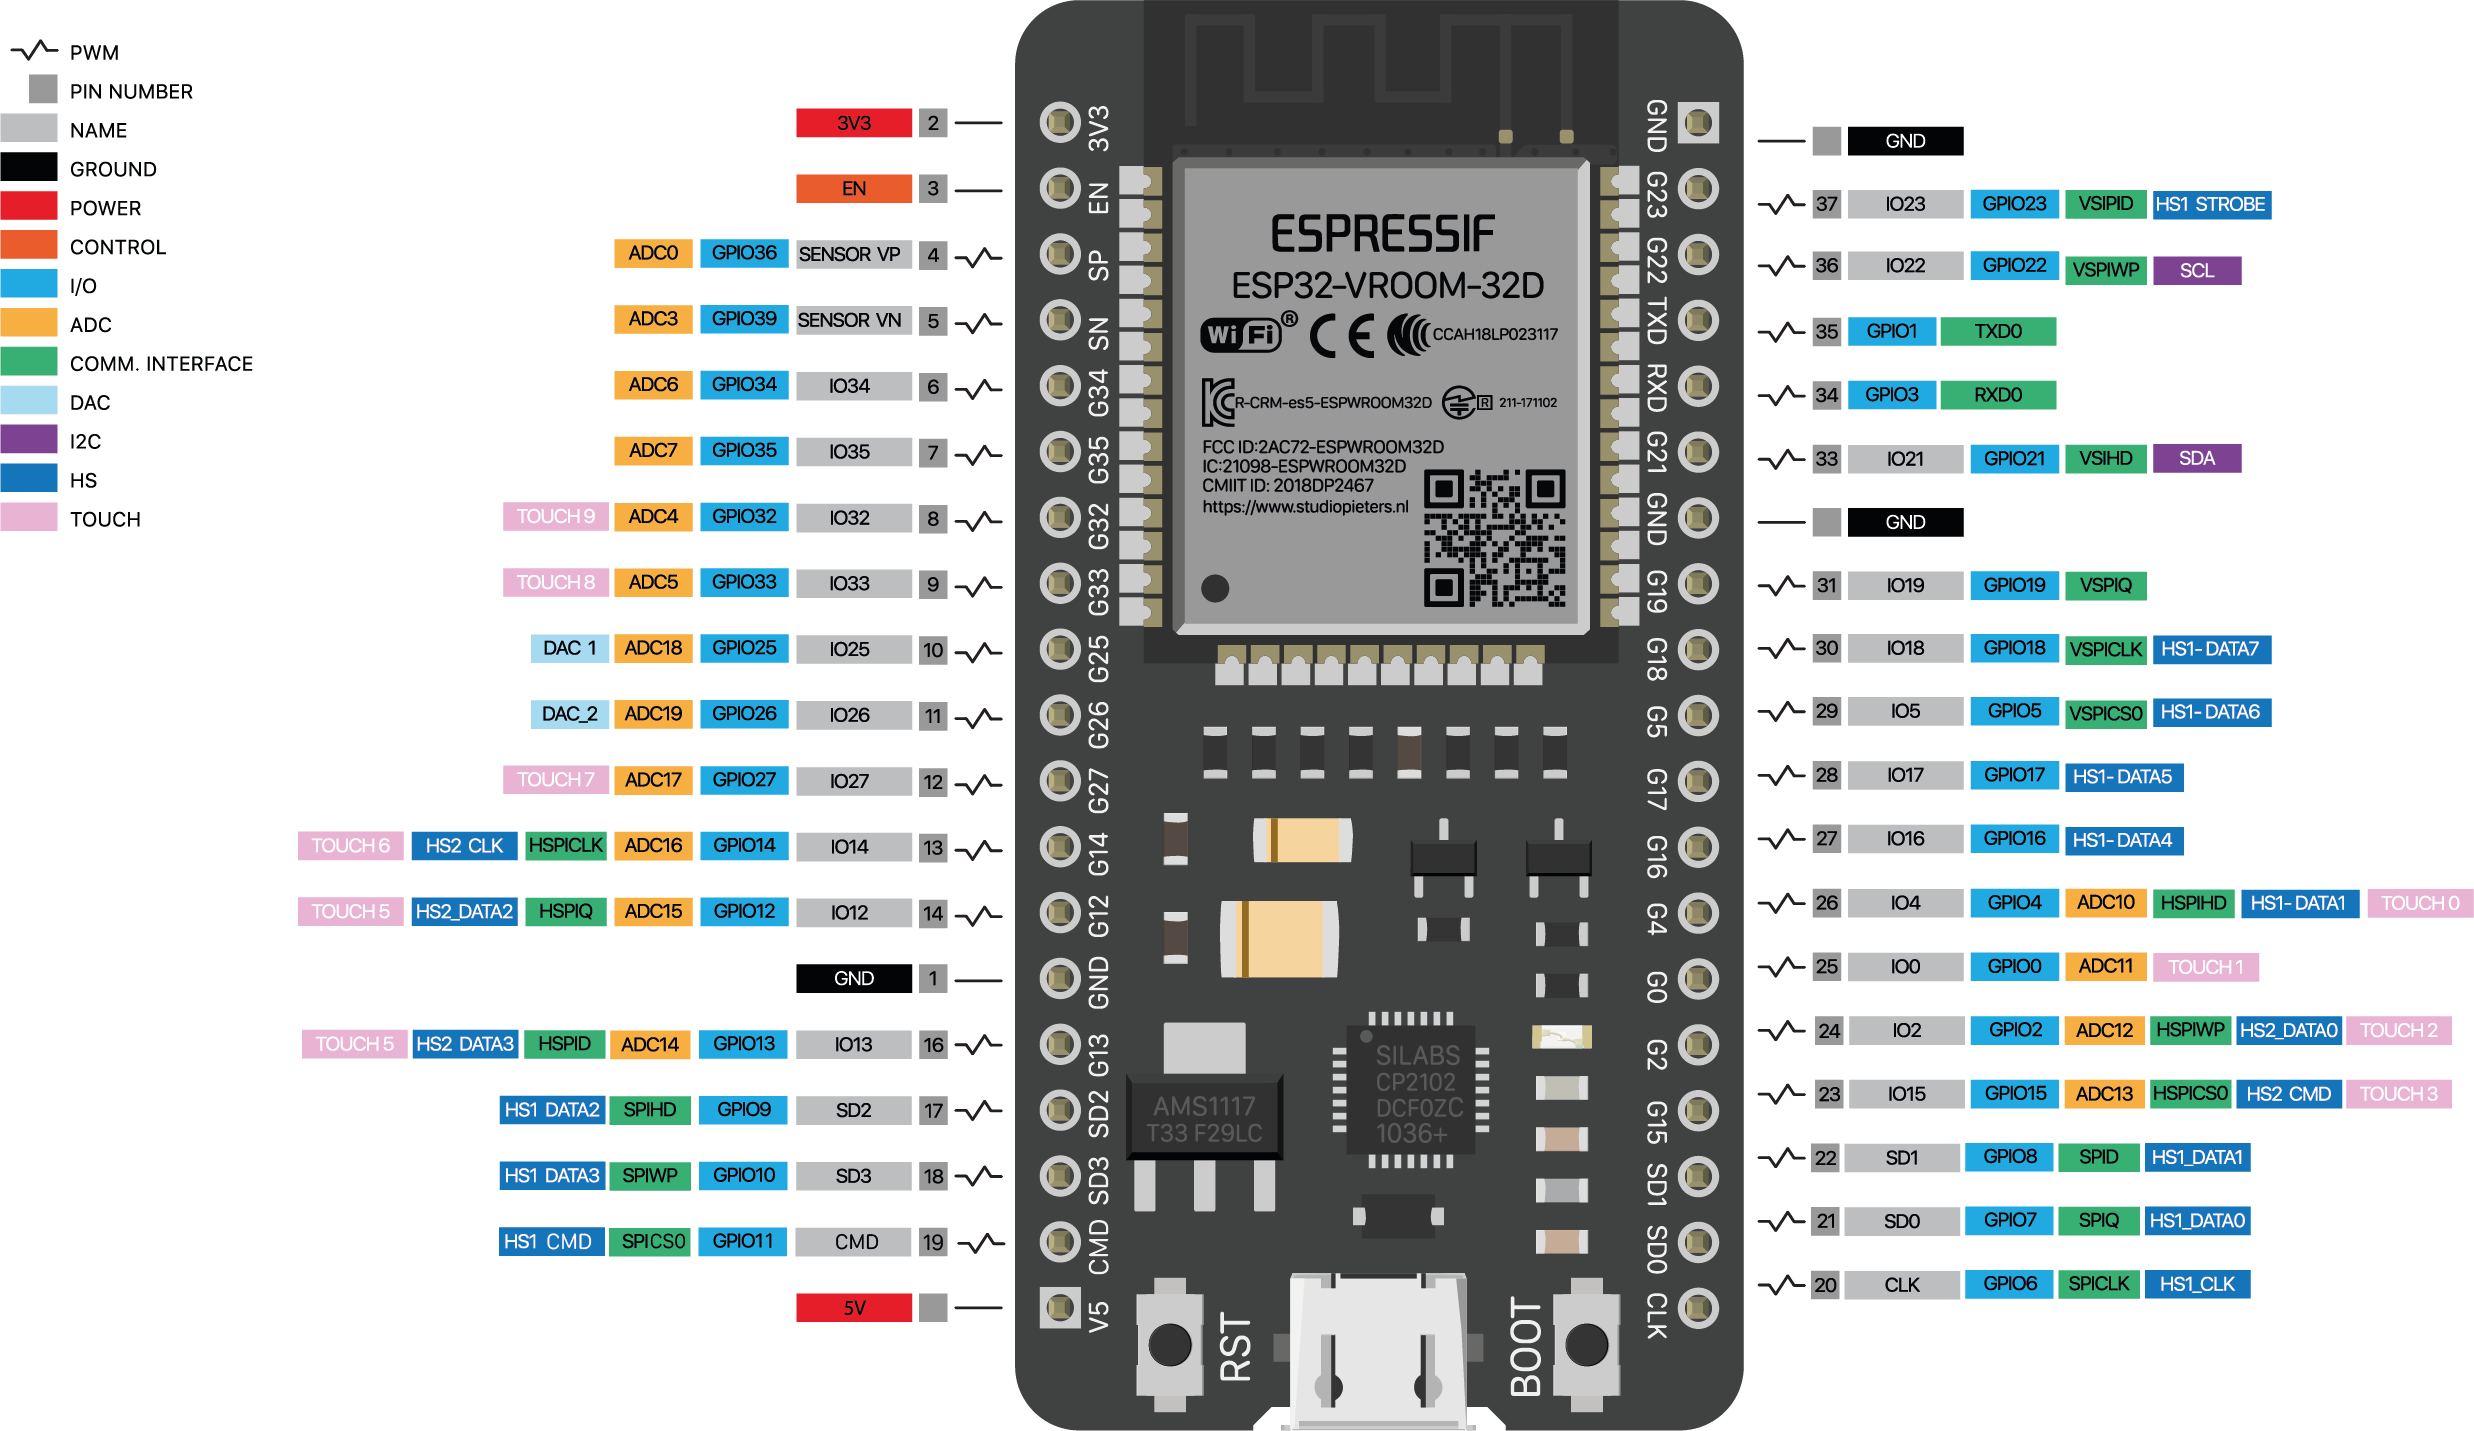
\includegraphics[width=0.5\textwidth]{imagenes/esp32.png}
	\caption{ESP32 pin layout\cite{esp32_img}}
\end{figure}

\section{Micropython}
Micropython \cite{ref12} es una implementación sencilla y eficiente de Python 3 para microcontroladores y otros entornos restringidos. Incluye un pequeño subconjunto de la biblioteca estándar de Python, y se puede extender fácilmente con módulos escritos en C. Micropython es un lenguaje de programación de alto nivel, por lo que es muy sencillo de programar. El firmware de Micropython es muy ligero, por lo que tan solo necesitamos 256Kb de memoria flash y 16Kb de RAM para poder ejecutarlo. \\

Ejemplo de como cambiar el valor de un pin digital\cite{ref13}:
\begin{lstlisting}[language=Python]
from machine import Pin

p0 = Pin(0, Pin.OUT)    # create output pin on GPIO0
p0.on()                 # set pin to "on" (high) level
p0.off()                # set pin to "off" (low) level
p0.value(1)             # set pin to on/high

p2 = Pin(2, Pin.IN)     # create input pin on GPIO2
print(p2.value())       # get value, 0 or 1

p4 = Pin(4, Pin.IN, Pin.PULL_UP) # enable internal pull-up resistor
p5 = Pin(5, Pin.OUT, value=1) # set pin high on creation
p6 = Pin(6, Pin.OUT, drive=Pin.DRIVE_3) # set maximum drive strength

\end{lstlisting}
\section{Comunicaciones inalámbricas en IoT}
Uno de los objetivos principales de este proyecto es poder enviar los datos que recoge cada sensor de corriente a un servidor para que se puedan procesar, analizar y mostrar en conjunto. Para ello, necesitamos alguna forma de comunicación inalámbrica. \\
\subsection{MQTT}
MQTT (Message Queuing Telemetry Transport) \cite{ref14} es un protocolo de mensajería ligero que se utiliza para la comunicación entre dispositivos en IoT. MQTT es un protocolo de publicación/ suscripción, por lo que los dispositivos se suscriben a un topic y los mensajes se publican en ese topic. \\

Caracteristicas principales:
\begin{itemize}
	\item Ligero y eficiente. Los clientes necesitas pocos recursos para poder usar el protocolo, lo que lo hace ideal para usarlo en microcontroladores.
	\item Comunicación bidireccional. Los clientes pueden publicar y suscribirse a topics.
	\item Es un protocolo muy escalable.
	\item Seguridad. MQTT permite el uso de TLS para encriptar la comunicación o el uso de protocolos de autenticación.
	\item Fiabilidad en la entrega de mensajes. MQTT permite especificar el nivel de fiabilidad(Quality of Service) en diferentes niveles. 
\end{itemize}
\begin{figure}[h!]
	\centering
	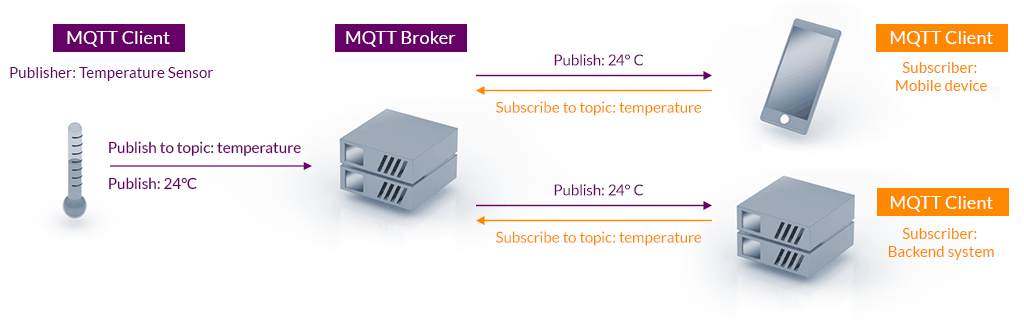
\includegraphics[width=0.75\textwidth]{imagenes/mqtt.png}
	\caption{Ejemplo de dispositivos comunicados por MQTT\cite{mqtt_img}}
\end{figure}

Es importante destacar la importancia del broker en MQTT. El broker es el encargado de recibir los mensajes de los clientes y reenviarlos a los clientes suscritos al topic. \\

\subsection{Zigbee}
Zigbee\cite{ref15} es un estandar de comunicación inalámbrica que se utiliza para la comunicación entre dispositivos en IoT. Zigbee es un protocolo de red mesh, por lo que los dispositivos se comunican entre ellos y no con un broker central a diferencia de MQTT.\\

En Zigbee, podemos encontrar tres clases diferentes de dispositivos:
\begin{itemize}
	\item Zigbee coordinator: El el dispositivo mas capaz encargado de administrar la red y de coordinar la comunicación entre los dispositivos.
	\item Zigbee router: Es un dispositivo que se encarga de reenviar los mensajes de los dispositivos a otros dispositivos ademas de correr su propia aplicación
	\item Zigbee end device: Contiene lo basico para poder comunicarse con un nodo padre y correr su propia aplicación.
\end{itemize}
\begin{figure}[h!]
	\centering
	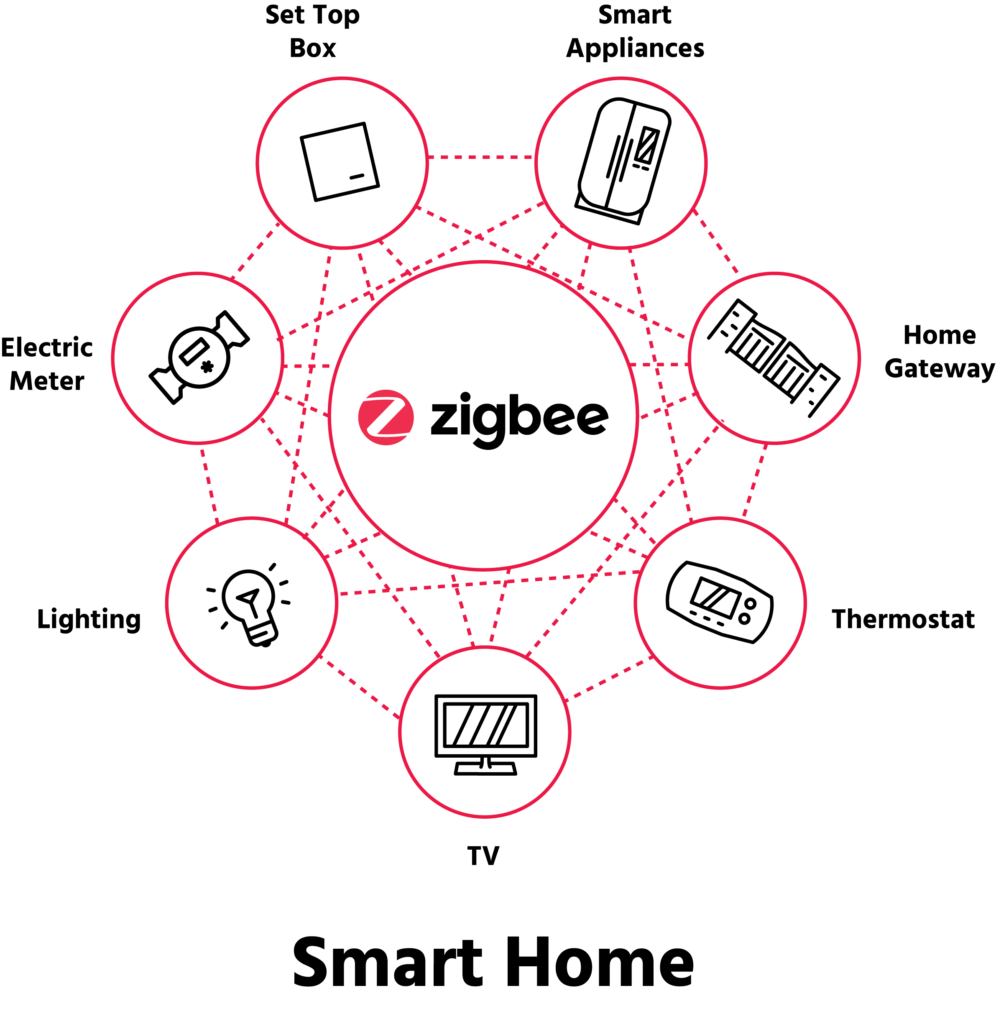
\includegraphics[width=0.45\textwidth]{imagenes/zigbee.png}
	\caption{Ejemplo de dispositivos comunicados por Zigbee\cite{zigbee_img}}
\end{figure}
Caracteristicas principales:
\begin{itemize}
	\item Es un protocolo de red mesh.
	\item Protocolo de bajo consumo, baja latencia y bajo coste.
	\item Es un protocolo de baja potencia, por lo que es ideal para usarlo en dispositivos que necesitan una comunicación a corta distancia.
	\item Hasta 65000 nodos en una red.
	\item Soporta encriptación AES-128.
\end{itemize}
\end{titlepage}
